% Template for articles for CCR (Computational Communication Research)
% Version 0.02

% This file contains information such as author, title, etc.
% Edit the body.tex file to add the contents (or change the \input{body} below)

\documentclass{ccr}

% Note - lines starting with a % are completely ignored by latex and function as comments
% See https://www.overleaf.com/read/hmwdsgcqkxrd for a complete example article

% The first part of the latex document contains metadata

% Regular metadata (title, authors etc)
\title{Project Report - Group 100}
\shorttitle{Project Report}
\authorsnames{Bogdan Paramon, Yair Chizi, Harald Toth}
% Short author list for footer
\shortauthors{Bogdan Paramon, Yair Chizi \& Harald Toth}

% Note that you need to provide as many affiliations as authors
% If multiple authors have the same affiliation, please copy that record as needed

% I used it for the student IDs.
\authorsaffiliations{
  5741513,
  5736668,
  5710812,
}


% You can add or rename the bibliography file(s) here
% Note that you can exported them from endnote or zotero directly and upload them to overleaf
\addbibresource{bibliography.bib}



% some packages that are generally useful when writing articles in latex
\usepackage{tabularx}  % for full-width tables
\usepackage{booktabs}  % for nicer horizontal lines in tables
\usepackage[mode=text]{siunitx} % for centering columns on the decimal mark
\usepackage{graphicx} % for including figures
\usepackage{csquotes}\MakeOuterQuote{"}  % to allow "double quotes" instead of ``double quote''
\usepackage[hidelinks]{hyperref} % for URLs and other hyperlinks


\begin{document}
\maketitle

% Include the body
% Note: You can also type it directly here, or include a file per section, whatever works best for you
% Any part of the report that relates to the basic features.
\section{Basic Features}
\subsection{BVH performance test}
Text Text Text...
\subsection{Light transparency sampling}
The algorithm suffers from two main problems. Firstly, in a scenario where an opaque object directly obstructs, no light is computed even if reflective surfaces around produce incident secondary rays. Secondly, only the obstruction of thin boundary surfaces contributes to the computation, with no consideration to obstructing object's internal medium.
\subsection{Depth of field}
Description:
The method iterates through all the pixels on the screen and calculates the position of the focal point relative to each pixel. It then generates several rays that start from a random location inside the pixel and end at the focal point. It calculates the color that results from the rays and averages their sum, which will be the final color of the pixel.

Visual debug:
There are three sliders in the depth of field section of the GUI: focal length, lens size, and number of samples. Focal length adjusts the distance from the camera to the focal point. Lens size modifies the maximum offset from the center of each pixel to the starting position of each ray. The number of samples specifies how many rays should be generated.

Location:
The method that implements depth of field is called renderImageWithDepthOfField and is located in the extra.cpp file. The only other changes related to this feature were made in main.cpp and common.h for the sliders in the GUI.


\includegraphics[]{Report - Group 100\\rsc\\dof_render1.png}

\includegraphics[]{Report - Group 100\\rsc\\dof_render2.png}
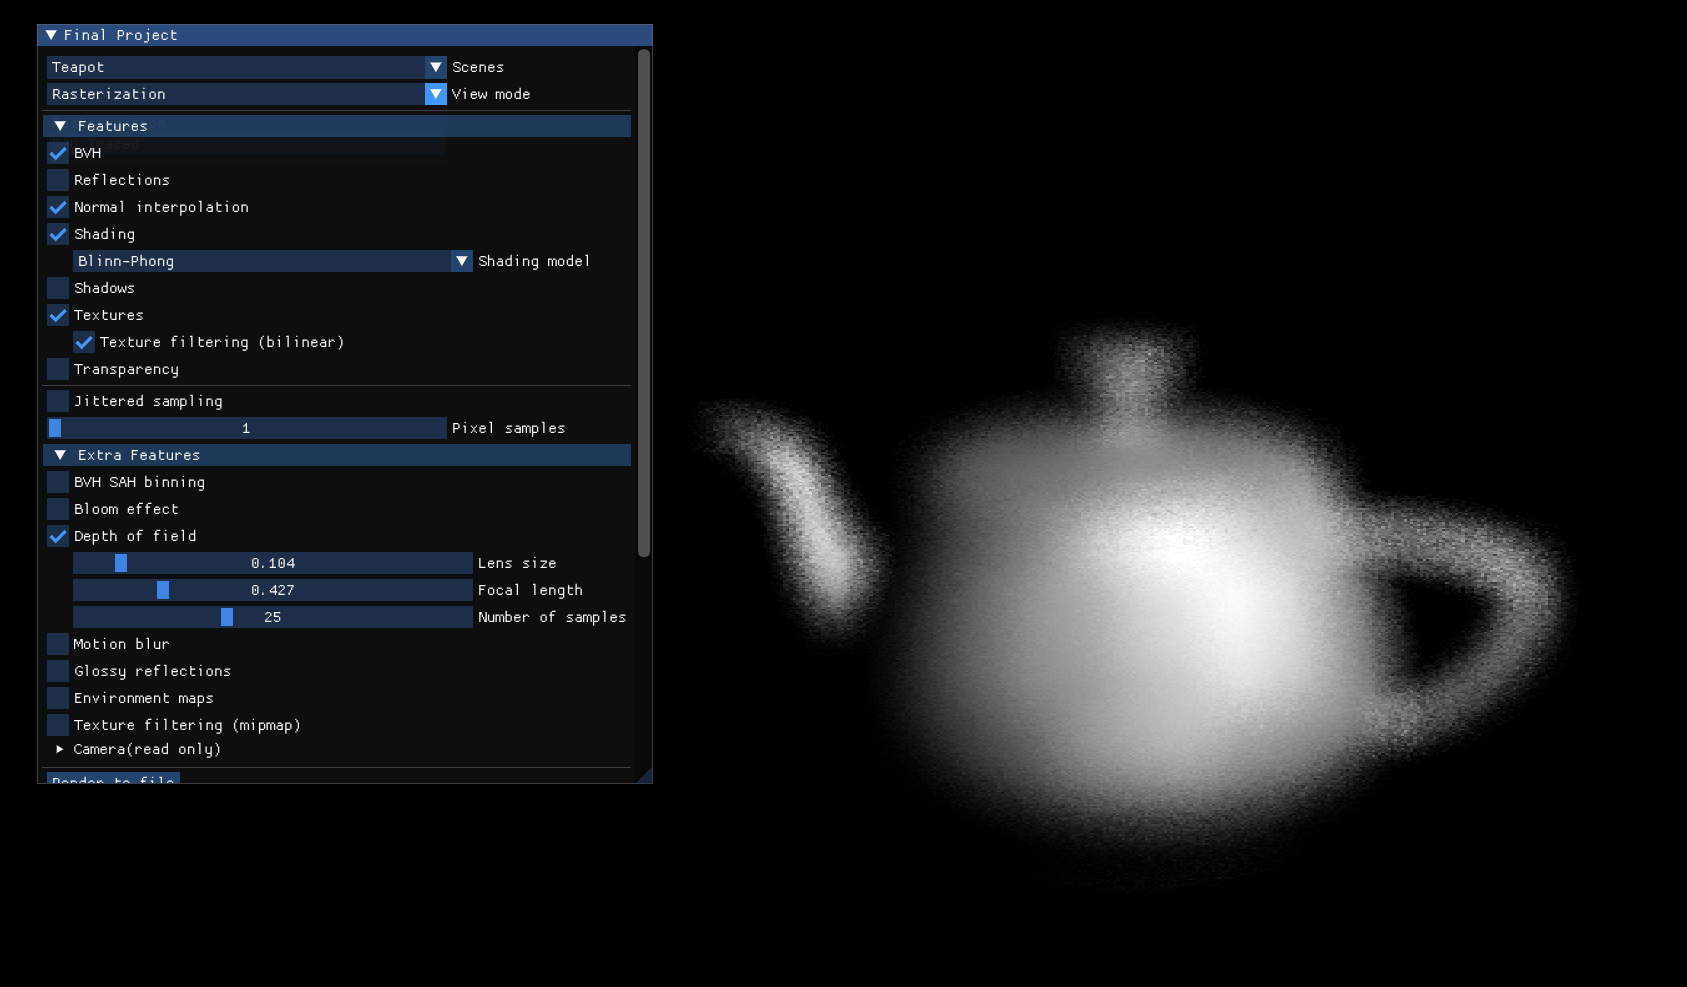
\includegraphics[]{Report - Group 100\\rsc\\dof_render3.png}

% Bibliography

% Uncomment the next line (\nocite{*}) if you want to include all items from your .bib file
% (e.g. if you didn't use the \textcite or \parencite commands above)
% \nocite{*}

% This command generates the bibliography
\printbibliography


\end{document}

